\section{指数矩上界}
\label{sec:tail-exponential-moments}

上一节看到，对高斯分布，阈值越远就要用越高阶的矩，而每次都要在许多阶之间挑选。能否一次把所有阶的矩都用上？指数函数的幂级数
\[
 \mathrm{e}^{\lambda x}=\sum_{k\geq0}\frac{\lambda^kx^k}{k!}
\]
恰好把各阶幂次按权重$\lambda^k/k!$加在一起。用$\mathrm{e}^{\lambda x}$去压尾事件的示性函数，得到的界只依赖一个期望。

\paragraph{矩母函数}
先给这个期望一个名字。它对有些$\lambda$有限，对有些$\lambda$可能是$+\infty$，所以同时记录它在哪里有限。

\begin{definition}[矩母函数]
\label{def:tail-mgf}
随机变量$X$的\term{矩母函数}（moment generating function）是
\begin{equation}
 M_X(\lambda)=\mathbb{E}\bigl[\mathrm{e}^{\lambda X}\bigr],\qquad \lambda\in\mathbb{R},
 \label{eq:tail-mgf}
\end{equation}
其中$\mathrm{e}^{\lambda X}>0$，期望总有定义，取值在$(0,+\infty]$中。
\end{definition}

总有$M_X(0)=1$。若$M_X(\lambda)$在$0$附近有限，把$\mathrm{e}^{\lambda X}$按幂级数展开并逐项取期望，$\lambda^k$的系数正是$\mathbb{E}[X^k]/k!$，这就是“矩母”这个名字的来历。逐项取期望的合理性以及矩母函数怎样识别分布，在第~\ref{chap:weak-convergence-of-distributions}章讨论；本节只把$M_X(\lambda)$当作一个可以计算的期望来用。

\paragraph{指数矩上界}
函数$x\mapsto\mathrm{e}^{\lambda x}$在$\lambda>0$时正且严格增，满足引理~\ref{lem:tail-markov-general}的全部条件，并且不要求$X$非负。

\begin{theorem}[指数矩上界]
\label{thm:tail-chernoff}
设$\lambda>0$，$M_X(\lambda)<\infty$。则对每个$t\in\mathbb{R}$，
\begin{equation}
 \mathbb{P}(X\geq t)\leq\mathrm{e}^{-\lambda t}M_X(\lambda) .
 \label{eq:tail-chernoff-lambda}
\end{equation}
因而
\begin{equation}
 \mathbb{P}(X\geq t)\leq\inf_{\lambda>0}\mathrm{e}^{-\lambda t}M_X(\lambda) ,
 \label{eq:tail-chernoff}
\end{equation}
其中$M_X(\lambda)=+\infty$的$\lambda$不起作用。
\end{theorem}

\begin{proof}
在引理~\ref{lem:tail-markov-general}中取$g(x)=\mathrm{e}^{\lambda x}$。它非负、不减，$g(t)=\mathrm{e}^{\lambda t}>0$，$\mathbb{E}[g(X)]=M_X(\lambda)<\infty$，所以
\[
 \mathbb{P}(X\geq t)\leq\frac{M_X(\lambda)}{\mathrm{e}^{\lambda t}}=\mathrm{e}^{-\lambda t}M_X(\lambda) .
\]
左边不依赖$\lambda$，对所有使右边有限的$\lambda>0$取下确界，得到式~\eqref{eq:tail-chernoff}。
\end{proof}

式~\eqref{eq:tail-chernoff}称为\term{Chernoff界}（Chernoff bound）。图~\ref{fig:tail-dominating}(c)是它的压法：$\mathrm{e}^{\lambda(x-t)}$在$x\geq t$时不小于$1$，在$x<t$时为正。$\lambda$控制这条曲线的形状：$\lambda$大时曲线在$t$左边迅速趋于零，把近处的质量压得很小，但在$t$右边陡峭上升，把远处的质量放得很大；$\lambda$小时正好相反。最优的$\lambda$在两者之间折中。

取对数可以把式~\eqref{eq:tail-chernoff}写成指数形式。记$\psi_X(\lambda)=\ln M_X(\lambda)$，则
\begin{equation}
 \mathbb{P}(X\geq t)\leq\exp\Bigl(-\sup_{\lambda>0}\bigl(\lambda t-\psi_X(\lambda)\bigr)\Bigr) .
 \label{eq:tail-chernoff-exponent}
\end{equation}
在下面的例子中，$\lambda t-\psi_X(\lambda)$都可以求导找到最大点。

\paragraph{高斯分布}
先计算$Z\sim\mathcal{N}(0,1)$的矩母函数。把指数部分配方，$\lambda x-x^2/2=\lambda^2/2-(x-\lambda)^2/2$，于是
\[
 M_Z(\lambda)=\mathrm{e}^{\lambda^2/2}\int_{-\infty}^{\infty}\frac{1}{\sqrt{2\pi}}\mathrm{e}^{-(x-\lambda)^2/2}\,\mathrm{d}x=\mathrm{e}^{\lambda^2/2} .
\]
最后的积分是平移后的高斯密度，等于$1$。它对一切实数$\lambda$有限。

代入式~\eqref{eq:tail-chernoff-lambda}，对$t>0$，
\[
 \mathbb{P}(Z\geq t)\leq\mathrm{e}^{-\lambda t+\lambda^2/2} .
\]
指数$-\lambda t+\lambda^2/2$是$\lambda$的二次函数，在$\lambda=t$处取最小值$-t^2/2$。所以
\begin{equation}
 \mathbb{P}(Z\geq t)\leq\mathrm{e}^{-t^2/2},\qquad t>0 .
 \label{eq:tail-gauss-chernoff}
\end{equation}
对$X\sim\mathcal{N}(\mu,\sigma^2)$，写$X=\mu+\sigma Z$，事件$\{X-\mu\geq t\}$就是$\{Z\geq t/\sigma\}$，得到
\[
 \mathbb{P}(X-\mu\geq t)\leq\mathrm{e}^{-t^2/(2\sigma^2)},\qquad t>0 .
\]

图~\ref{fig:tail-chernoff-lambda}(b)画出$t=1,2,3$时的函数$\lambda\mapsto\mathrm{e}^{-\lambda t+\lambda^2/2}$，红点是最小点$\lambda=t$。三个最小值与精确值的对比是
\[
 \begin{gathered}
 t=1:\ 0.607\ \text{对}\ 0.1587,\qquad t=2:\ 0.135\ \text{对}\ 0.0228,\\
 t=3:\ 0.0111\ \text{对}\ 0.00135 .
 \end{gathered}
\]
精确值与上界之比依次约为$0.26$、$0.17$、$0.12$，变化缓慢；起主导作用的因子$\mathrm{e}^{-t^2/2}$被界完整地抓住了。与之相比，Chebyshev界$1/t^2$在$t=3$处是$0.111$，大了八十多倍。

\paragraph{贯穿例子}
对$X\sim\operatorname{Bin}(20,1/2)$，按定义求和并用二项式定理：
\[
 M_X(\lambda)=\sum_{k=0}^{20}\binom{20}{k}2^{-20}\mathrm{e}^{\lambda k}=\Bigl(\frac{1+\mathrm{e}^{\lambda}}{2}\Bigr)^{20} .
\]
在$t=15$处，要最小化的函数是
\[
 h(\lambda)=\ln\bigl(\mathrm{e}^{-15\lambda}M_X(\lambda)\bigr)=-15\lambda+20\ln(1+\mathrm{e}^{\lambda})-20\ln2 .
\]

对$\lambda$求导并令导数为零：
\[
 h'(\lambda)=-15+\frac{20\,\mathrm{e}^{\lambda}}{1+\mathrm{e}^{\lambda}}=0 .
\]
由$4\mathrm{e}^{\lambda}=3(1+\mathrm{e}^{\lambda})$解得
\[
 \mathrm{e}^{\lambda}=3,\qquad \lambda=\ln3\approx1.099 .
\]
再求一次导数，
\[
 h''(\lambda)=\frac{20\,\mathrm{e}^{\lambda}}{(1+\mathrm{e}^{\lambda})^2}>0 ,
\]
所以$h'$严格增，$\lambda=\ln3$是唯一的最小点。

代回去，$M_X(\ln3)=2^{20}$，$\mathrm{e}^{-15\ln3}=3^{-15}$，所以
\begin{equation}
 \mathbb{P}(X\geq15)\leq\frac{2^{20}}{3^{15}}=\frac{1048576}{14348907}\approx0.0731 .
 \label{eq:tail-binomial-chernoff}
\end{equation}
这比六阶矩界$0.108$更好，距精确值$0.0207$只差约$3.5$倍。图~\ref{fig:tail-chernoff-lambda}(a)显示了$\lambda$的选择：$\lambda$太小，指数函数几乎是常数，界接近$1$；$\lambda$太大，远处的质量被放得过大，界又上升。

\begin{BookInlineFigure}
 \centering
 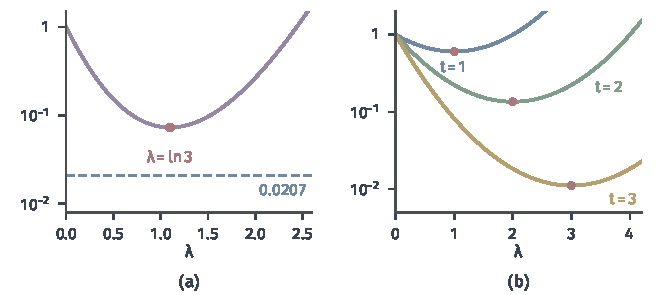
\includegraphics[width=112mm]{figures/07-probability/01-elementary-probability/matplotlib/tail-chernoff-lambda/figure.pdf}
 \caption{指数矩上界作为$\lambda$的函数，纵轴为对数刻度，红点为最小点。(a)$X\sim\operatorname{Bin}(20,1/2)$，$t=15$，紫线为$\mathrm{e}^{-15\lambda}M_X(\lambda)$，最小值$2^{20}/3^{15}\approx0.0731$在$\lambda=\ln3$处取到，蓝色虚线为精确值$0.0207$。(b)$Z\sim\mathcal{N}(0,1)$，$t=1,2,3$时的$\mathrm{e}^{-\lambda t+\lambda^2/2}$，最小点为$\lambda=t$。}
 \label{fig:tail-chernoff-lambda}
\end{BookInlineFigure}

同样的计算适用于一般的二项分布。设$X\sim\operatorname{Bin}(n,p)$，$0<p<1$，阈值写成$na$，$p<a<1$。$M_X(\lambda)=(1-p+p\mathrm{e}^{\lambda})^n$，令导数为零得$\mathrm{e}^{\lambda}=a(1-p)/\bigl(p(1-a)\bigr)$，它大于$1$，所以$\lambda>0$。代回整理，得到
\begin{equation}
 \mathbb{P}(X\geq na)\leq\Bigl[\Bigl(\frac{p}{a}\Bigr)^{a}\Bigl(\frac{1-p}{1-a}\Bigr)^{1-a}\Bigr]^{n} .
 \label{eq:tail-binomial-chernoff-general}
\end{equation}
方括号里的数小于$1$。比例$a$固定时，界随试验次数$n$按几何级数缩小。取$n=20$，$p=1/2$，$a=3/4$，方括号里是$(2/3)^{3/4}2^{1/4}\approx0.8774$，其$20$次方回到$0.0731$。

\paragraph{指数分布}
对$X\sim\operatorname{Exp}(1)$，矩母函数是
\[
 M_X(\lambda)=\int_0^{\infty}\mathrm{e}^{\lambda x}\mathrm{e}^{-x}\,\mathrm{d}x=\begin{cases}\dfrac{1}{1-\lambda}, & \lambda<1,\\ +\infty, & \lambda\geq1 .\end{cases}
\]
$\lambda\geq1$时被积函数不趋于零，积分发散。所以下确界只能在$0<\lambda<1$中取。

对$t>1$，取对数后要最小化的是
\[
 \ln\frac{\mathrm{e}^{-\lambda t}}{1-\lambda}=-\lambda t-\ln(1-\lambda),\qquad 0<\lambda<1 .
\]
它的导数为$-t+1/(1-\lambda)$，零点是$\lambda=1-1/t\in(0,1)$，导数在它左边为负、右边为正。代回得
\begin{equation}
 \mathbb{P}(X\geq t)\leq t\,\mathrm{e}^{1-t},\qquad t>1 .
 \label{eq:tail-exp-chernoff}
\end{equation}
$t\leq1$时导数在$(0,1)$上处处非负，下确界在$\lambda\to0$时取到，界为$1$。

精确值是$\mathrm{e}^{-t}$，两者之比为$\mathrm{e}\,t$：$t=5$时界为$0.0916$，精确值为$0.0067$。指数衰减率$\mathrm{e}^{-t}$被保留了，丢掉的是一个线性因子。原因是$\lambda$不能取到$1$：要完全抓住$\mathrm{e}^{-t}$，需要$\lambda=1$，而那里矩母函数已经是无穷。图~\ref{fig:tail-chernoff-compare}把两个模型上的指数矩上界与较弱的界放在一起。

\begin{BookInlineFigure}
 \centering
 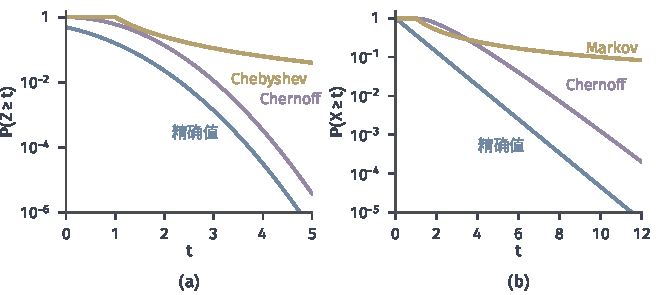
\includegraphics[width=112mm]{figures/07-probability/01-elementary-probability/matplotlib/tail-chernoff-compare/figure.pdf}
 \caption{精确右尾（蓝线）、指数矩上界（紫线）与矩上界（黄线），纵轴为对数刻度。(a)$Z\sim\mathcal{N}(0,1)$：$Q(t)$，$\mathrm{e}^{-t^2/2}$，Chebyshev界$\min\{1,1/t^2\}$。(b)$X\sim\operatorname{Exp}(1)$：$\mathrm{e}^{-t}$，$\min\{1,t\,\mathrm{e}^{1-t}\}$，Markov界$\min\{1,1/t\}$。}
 \label{fig:tail-chernoff-compare}
\end{BookInlineFigure}

\paragraph{指数矩有限与尾部指数衰减}
指数分布的例子说明，矩母函数在哪里有限，与尾部衰减得多快直接相关。图~\ref{fig:tail-mgf-domain}画出三个矩母函数：高斯分布的$\mathrm{e}^{\lambda^2/2}$处处有限；$\operatorname{Exp}(1)$的$1/(1-\lambda)$在$\lambda\to1$时趋于无穷；尺度为$1$的Laplace分布，按同样的积分得$1/(1-\lambda^2)$，只在$\lvert\lambda\rvert<1$时有限。

\begin{BookInlineFigure}
 \centering
 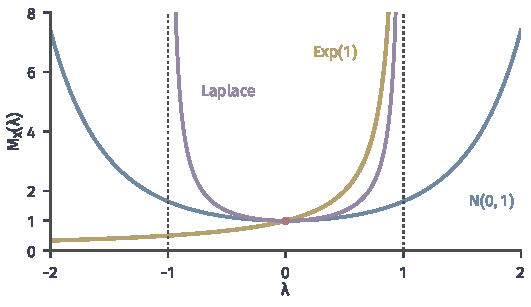
\includegraphics[width=90mm]{figures/07-probability/01-elementary-probability/matplotlib/tail-mgf-domain/figure.pdf}
 \caption{三个矩母函数。蓝线为$\mathcal{N}(0,1)$的$\mathrm{e}^{\lambda^2/2}$，黄线为$\operatorname{Exp}(1)$的$1/(1-\lambda)$（$\lambda<1$），紫线为尺度$1$的Laplace分布的$1/(1-\lambda^2)$（$\lvert\lambda\rvert<1$）。点线标出$\lambda=\pm1$，红点为所有矩母函数共有的$M_X(0)=1$。}
 \label{fig:tail-mgf-domain}
\end{BookInlineFigure}

一个方向已经由式~\eqref{eq:tail-chernoff-lambda}给出：只要某个$\lambda_0>0$使$M_X(\lambda_0)<\infty$，右尾就至少按$\mathrm{e}^{-\lambda_0t}$衰减。对非负、有密度的变量，反方向也成立。

\begin{theorem}[指数矩与尾部衰减]
\label{thm:tail-mgf-decay}
设$X\geq0$有密度，存在常数$C>0$、$c>0$，使$\mathbb{P}(X>s)\leq C\mathrm{e}^{-cs}$对一切$s\geq0$成立。则对$0\leq\lambda<c$，
\begin{equation}
 M_X(\lambda)\leq1+\frac{C\lambda}{c-\lambda}<\infty .
 \label{eq:tail-mgf-decay}
\end{equation}
\end{theorem}

\begin{proof}
在引理~\ref{lem:tail-integral}中取$g(s)=\mathrm{e}^{\lambda s}$，它连续可微且不减，$g(0)=1$，$g'(s)=\lambda\mathrm{e}^{\lambda s}$。于是
\[
 M_X(\lambda)=1+\int_0^{\infty}\lambda\mathrm{e}^{\lambda s}\,\mathbb{P}(X>s)\,\mathrm{d}s .
\]
代入尾部的假设，积分不超过
\[
 \int_0^{\infty}\lambda\mathrm{e}^{\lambda s}\,C\mathrm{e}^{-cs}\,\mathrm{d}s=C\lambda\int_0^{\infty}\mathrm{e}^{-(c-\lambda)s}\,\mathrm{d}s=\frac{C\lambda}{c-\lambda} .
\]
最后一步用到$c-\lambda>0$。
\end{proof}

对$\operatorname{Exp}(1)$，$C=c=1$，式~\eqref{eq:tail-mgf-decay}给出$1+\lambda/(1-\lambda)=1/(1-\lambda)$，与直接计算的结果相同。

\paragraph{重尾时没有指数矩}
尾部只按幂次衰减时，矩母函数在$\lambda>0$处全是无穷。对$\alpha=3$的Pareto分布，由幂级数的一项，$x\geq0$时$\mathrm{e}^{\lambda x}\geq(\lambda x)^3/6$，所以
\[
 M_X(\lambda)\geq\frac{\lambda^3}{6}\,\mathbb{E}[X^3]=+\infty,\qquad \lambda>0 .
\]
三阶矩已经无穷，指数矩更不可能有限。自由度有限的t分布、Cauchy分布也是如此。对这类分布，式~\eqref{eq:tail-chernoff}的下确界里没有任何可用的$\lambda$，只能退回到存在的那些矩。尾部按幂次衰减的分布通常称为\term{重尾分布}（heavy-tailed distribution），它们的矩上界在下一节单独检查。

\paragraph{左尾与双侧}
对左尾，把定理用于$-X$。对$\lambda>0$，事件$\{X\leq t\}$就是$\{-X\geq-t\}$，而$-X$在$\lambda$处的矩母函数是$M_X(-\lambda)$，于是
\begin{equation}
 \mathbb{P}(X\leq t)\leq\inf_{\lambda>0}\mathrm{e}^{\lambda t}M_X(-\lambda) .
 \label{eq:tail-chernoff-left}
\end{equation}
双侧事件按式~\eqref{eq:tail-two-sided}拆成两侧，各用一个界后相加。标准高斯分布关于$0$对称，两侧的界相同，得
\[
 \mathbb{P}(\lvert Z\rvert\geq t)\leq2\mathrm{e}^{-t^2/2},\qquad t>0 .
\]

\paragraph{本节的边界}
这里只用了单个随机变量的矩母函数。矩母函数还有两方面的用途：在一定条件下它决定分布本身，这类识别工具在第~\ref{chap:weak-convergence-of-distributions}章介绍；对许多独立量之和，它可以分解成各项矩母函数的乘积，于是式~\eqref{eq:tail-chernoff}给出样本平均偏离均值的指数界，可参考\BookChapterRef{chap:finite-sample-error-bounds}{卷八第4章“有限样本的误差上界”}。
